\chapter{Conclusiones}
\label{cap:capitulo5}
En este capítulo se realiza una recapitulación de los problemas resueltos y las soluciones utilizadas, así como los experiementos realizados para validar los resultados. Por último, se citan una serie de posibles usos alternativos del software utilizado.\\

\section{Conclusiones}
\label{section:conclusiones}
El objetivo principal era implementar un coche autónomo bajo una plataforma de bajo coste y reducido tamaño capaz de circular por un circuito o carretera en un entorno dinámico interactuando con objetos propios de una ciudad, como semáforos, señales de stop o peatones. Dicho objetivo debía ser llevado a cabo en dos entornos distintos; en un entorno simulado utilizando el simulador \textit{Gazebo}\footnote{\url{https://github.com/gazebosim/gz-sim}} y en un entorno real, ensamblando un robot donde se utiliza como cerebro, una placa \textit{NVIDIA Jetson Nano}\footnote{\url{https://developer.nvidia.com/embedded/jetson-nano}} y como sensor principal, una cámara USB.\\

Para cumplir dichos objetivos, se han utilizado dos redes neuronales. Por un lado, para realizar el seguimiento de carril, se ha hecho uso de la librería \textit{JetRacer}\footnote{\url{https://github.com/NVIDIA-AI-IOT/jetracer}}. Dicha librería implementa una red residual, concretamente la red preentrenada \textit{ResNet-18}, que mediante un entrenamiento previo a partir de un \textit{dataset} propio, proporciona como salida de la red, el centro del carril o carretera. Dicha salida se utiliza como entrada en un controlador implementado para poder seguir recto o girar en caso de enfrentarse a una curva.

Por otro lado, se ha utilizado la red \textit{YOLO V3 Tiny} mediante el \textit{framework} \textit{Darknet}\footnote{\url{https://pjreddie.com/darknet/}} y su implementación en \textit{ROS}, \textit{Darknet ROS} para la detección de objetos. En el caso del entorno real, la red mencionada ha sido entrenada a través de un \textit{dataset} propio con los objetos reales, con el objetivo de ofrecer una detección de mayor fiabilidad. 

Todo ello ha sido combinado en dos paquetes \textit{ROS}, diferenciando entorno simulado y real.\\

La principal limitación del sistema es la potencia de la placa utilizada. Al necesitar dos redes neuronales y para obtener un rendimiento aceptable, es necesario trabajar con una resolución considerablemente baja. Por otra parte, al disponer de una sola cámara esta debe tener un ángulo de inclinación hacia abajo para poder visualizar correctamente el circuito, lo que provoca un campo de visión reducido que limita la detección de objetos de gran altura.\\

\section{Líneas futuras}
\label{section:future}
Tal y como se expuso en el Capítulo 1, exiten multitud de casos donde se utilizan vehículos autónomos, y no únicamente en el ámbito de la conducción. Por lo que la solución implementada podría ser aplicable a otros usos.\\ 

Por ejemplo, en el ámbito de la inspección, la red neuronal de seguimiento de carril podría ser utilizada para navegar a lo largo de un túnel, como el de la Figura \ref{fig:moreusages}, en el que buscan artefactos explosivos a través de la red de detección de objetos.\\

Otro posible utilidad sería la exploración de bosques o montañas para prevenir incendios de modo que el robot debería seguir la senda o camino en busca de fuego o signos de peligro haciendo uso de la detección de objetos para poder alertar correctamente.\\

\begin{figure} [h!]
	\begin{center}
		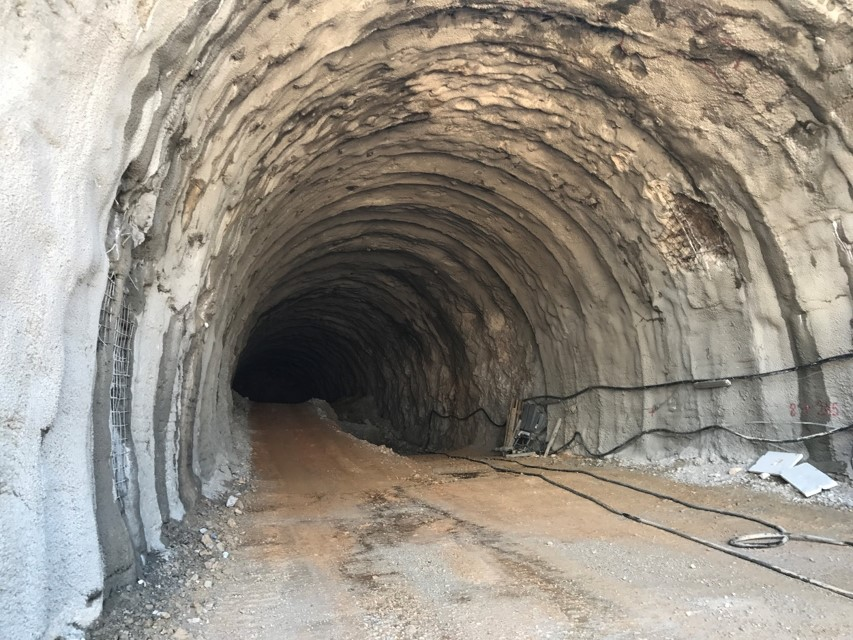
\includegraphics[width=5cm]{figs/tunel}\hspace{0.5cm}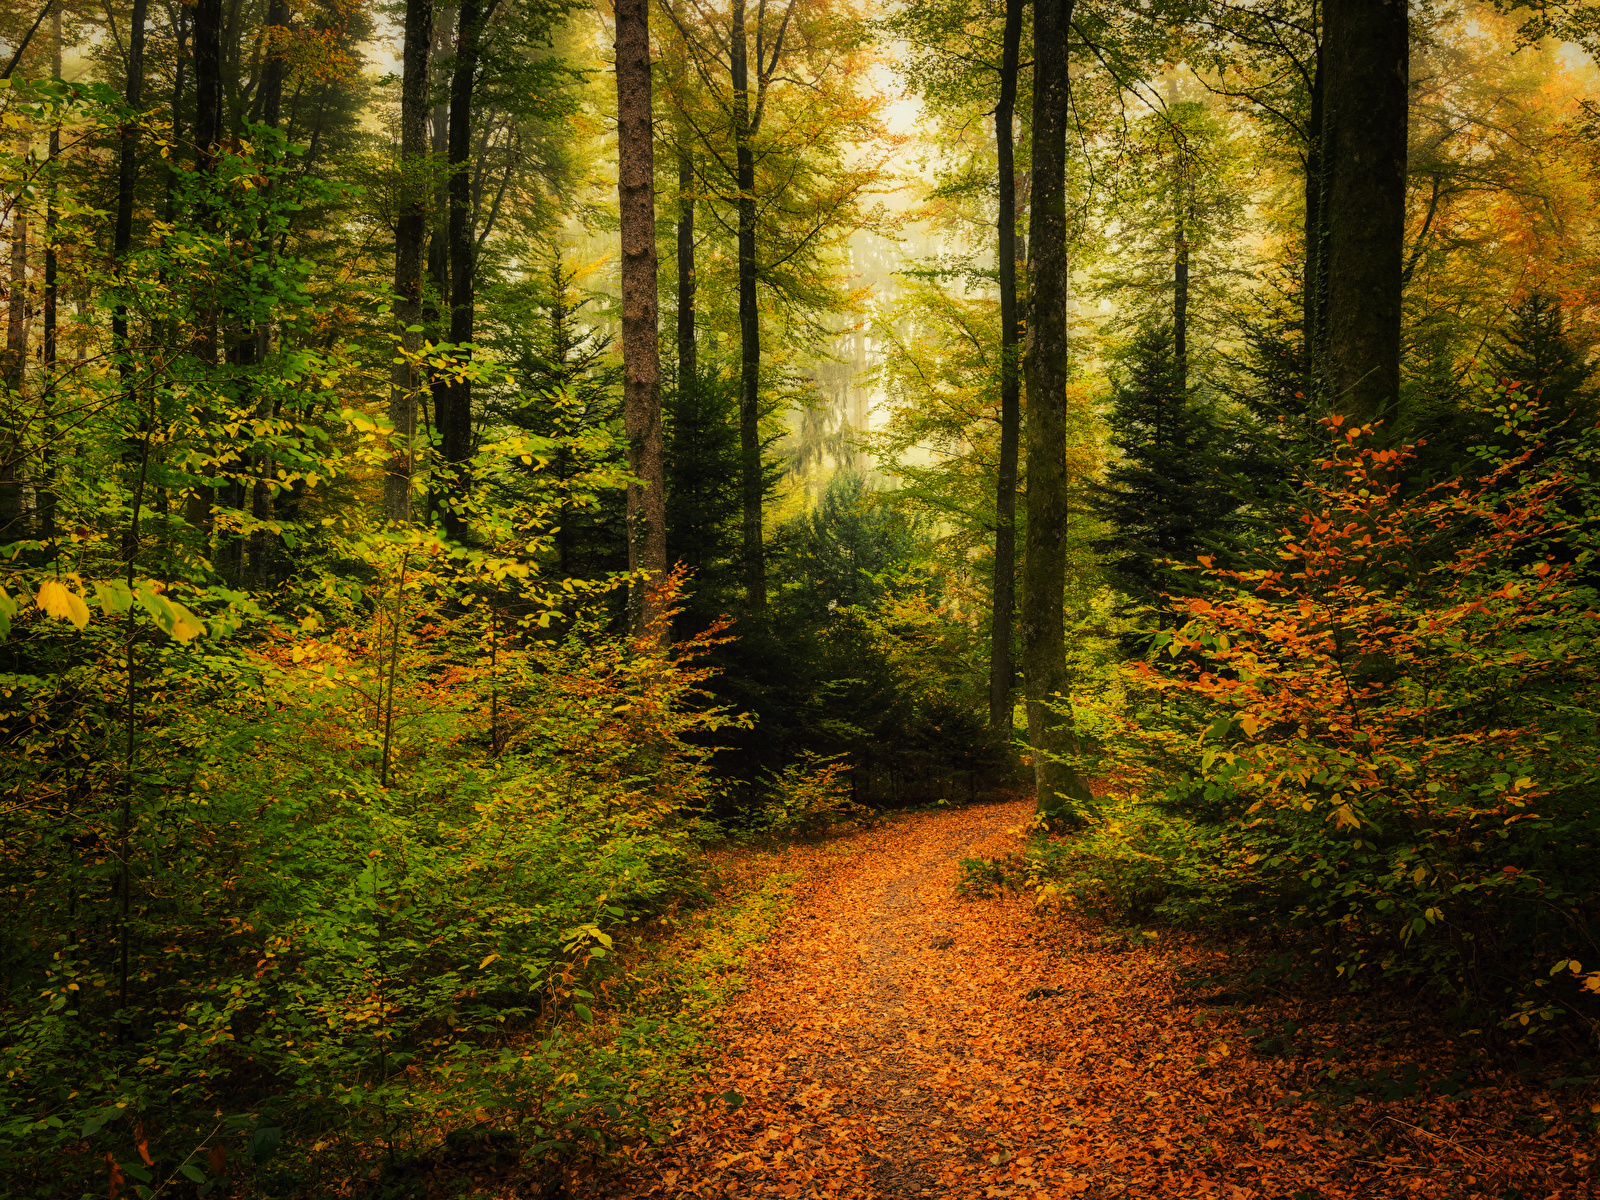
\includegraphics[width=5cm]{figs/forest}
	\end{center}
	\caption{Posibles usos alternativos del software implementado.}
	\label{fig:moreusages}
\end{figure}\

Todo ello son ámbitos de aplicación que no hacen más que proporcionar una intuición acerca del potencial de las redes neuronales, que mediante un entrenamiento a través de un conjunto grande y completo de datos, permiten adaptarse a multitud de situaciones.\\

% footnote images cite
% era o es
% que es red preentrenada
% requisitos implícitos